\documentclass[11pt]{article}
\usepackage[utf8]{inputenc}
\usepackage[T1]{fontenc}
\usepackage{natbib}
\usepackage{hyperref}
\usepackage{titling}
\usepackage[left=0.8in,right=0.8in,bottom=0.9in, top=0.9in]{geometry}
\usepackage{setspace}
\usepackage{amsmath}
\usepackage{amssymb}
\usepackage{graphicx}
\usepackage{float}
\usepackage{algorithm}
\usepackage{algpseudocode}
\usepackage{tikz}
\usetikzlibrary{positioning,fit,backgrounds, calc}


\setlength{\droptitle}{-7em}
\setstretch{1.1}

\title{Literature Summary}
\author{Damanveer Singh Dhaliwal}
\date{\today}

\begin{document}
\begin{center}
{\textbf{Regime-Switching Gaussian Process Cross-Sectional Asset Pricing with Covariate Driven Transitions} \\
STA2104 - Project \\[2pt]
Damanveer Singh Dhaliwal \quad Student ID: 1012787147 \quad d.dhaliwal@mail.utoronto.ca}
\end{center}

\section{Abstract}
The cross-section of expected stock returns is non-linear in firm characteristics and non-stationary across market environments. Yet existing models and papers only address one of these features at a time. In this paper, we propose a regime-switching Gaussian process cross-sectional pricing model with non-homogeneous transitions that will be driven by observable macroeconomic covariates such as the VIX, credit spread/term spread, inspired by economic intuition. The model will be fit via generalized EM algorithm that preserves the conditional independence required for exact forward-backward inference, conditional on the current emission likelihoods. The methodological contribution here is the integration of this macroeconomic covariate-driven transitions into non-parametric GP pricing models. The empirical contribution is an interpretable, non-parametric measure of characteristic importance recovered from regime-specific ARD lengthscales, showing which firm characteristics matter most for pricing stocks in each market environment. The proposed model was able to recover true lengthscales and identify the regime path on synthetic data, while on real monthly return data from 2000 to 2024. It underperformed linear and tree-based baseline models. However, it showed us that there are significant gains that can be isolated to the regime switching layer by outperforming the single regime GP. 

\section{Introduction}
The cross-section of expected stock returns involves modelling the returns of a large number of stocks at a given point in time. The central question in empirical finance is to understand why some stocks earn higher returns than others. This is modelled by the relationship between the expected stock returns and the relationship between firm characteristics such as size, value, momentum, and profitability; however, there are two specific challenges that arise when modelling this. 

First, the relationship is highly non-linear and involves economically important interactions among characteristics. \cite{gu_empirical_2020} document that machine learning methods capable of capturing non-linearity and interactions materially outperform the linear \cite{fama_risk_1973} framework. Second, the relationship is non-stationary. Characteristics that are priced in calm markets may cease to be priced in stress episodes and vice versa. Most existing cross-sectional models address one of these features at a time: either flexible functional forms with stationary parameters or simple functional forms with time-varying coefficients, but not both jointly. 

A probabilistic model with Gaussian process emissions is well motivated here for reasons that matter to a financial economist. First, regime membership is inherently uncertain. A statement like "there is 60\% probability we are in a high stress regime" requires a posterior distribution over latent states, not a point estimate. Second, the Gaussian process is uniquely suited to the within-regime pricing function. It captures non-linearity non-parametrically, and its closed-form posterior variance gives uncertainty bands on expected returns, where tree-based or neural approaches would require expensive bootstraps. The ARD kernel yields interpretable length scales that rank which firm characteristics matter in each regime. Third, probabilistic regime inference admits natural model averaging: $E[r_{i, t+1} | \mathcal{D}_t] = \sum_k P(s_t = k |\mathcal{D}_t) \cdot \mu_k(x_{i,t} | \mathcal{D}_t^{(k)})$ where $\mu_k$ is the regime-k GP posterior mean; it integrates over current regime uncertainty rather than conditioning on a point estimate. 

This paper proposes a new asset pricing model with three components: (1) a Gaussian process with an ARD kernel that learns the pricing function non-parametrically within each regime, (2) a Hidden Markov Model (HMM) governing latent regime dynamics, and (3) non-homogeneous transition probabilities that are driven by observable macroeconomic covariates including the VIX (volatility index), credit spreads (BAA-AAA), and the term spread. The number of regimes $K$ is fixed a priori at $K=2$ for computational efficiency and interpretability. 

The methodological contribution of this paper is the introduction of macro-driven regime transitions to the non-parametric GP pricing under a generalized EM algorithm that preserves the conditional independence required for exact forward-backward inference in the E-step. The empirical contribution follows directly: the regime-specific ARD lengthscales $\ell_k^{(j)}$ yield a principled non-parametric measure of which characteristics of a stock are most important for pricing in each market regime. We evaluate the model on synthetic data where ground truth is known and on monthly S\&P 500 returns from the year 2000 to 2024 using a rolling window out-of-sample design against the standard linear, tree-based, and single regime GP benchmarks.

\section{Formal Model}
\subsection{Overview}
The model captures three key empirical features of the cross-section of stock returns: nonlinearity in the mapping from firm characteristics to expected returns, shifting of that mapping across market environments, and transitions between market environments (regimes) driven by macroeconomic conditions. Let $r_{i,t+1}$ denote the excess return of stock $i$ from period $t$ to $t+1$, where $i=1,\dots,N_t$ indexes firms in the cross-section and $t=1,\dots,T$ indexes time. Let $x_{i,t} \in \mathbb{R}^p$ denote a vector of firm characteristics observed at time $t$, $X_t = [x_{1,t}, \dots, x_{N_t,t}]^\top$ the cross-sectional design matrix, and $z_{t-1}\in\mathbb{R}^m$ denote a vector of observable macroeconomic covariates. Firm characteristics use a six-month Compustat reporting lag and macroeconomic covariates entering the transition model are lagged one month. A latent regime variable $s_t \in \{0,1\}$ indexes the active market regime at time $t$, with $K = 2$ fixed a priori.

The pricing function is assumed to be a Gaussian process prior, motivated by the non-linearity in the characteristic return relation. The latent regime structure is motivated by time variation in the same relationship. The regime process itself follows macro-driven transition probabilities $P(s_t | s_{t-1} = k, z_{t-1})$ to capture the fact that macroeconomic conditions drive shifts in the underlying return-generating process. Figure 1 presents the full model in plate notation: shaded circles are observed, open circles are latent, and squares are parameters; the regime $s_t$ evolves as a non-homogeneous Markov chain driven by macro covariates $z_{t-1}$, and conditional on $s_t$, the cross-sectional return vector $r_{i,t+1}$ is drawn from a regime-specific GP indexed by characteristics $x_{i,t}$.

The arrow $z_{t-1} \to s_t$ encodes the non-homogeneous transition mechanism that distinguishes this model from a standard HMM-GP. Parameters $(\alpha,\beta)$ govern transition logits; $\theta_{GP}=\{\eta_k,\ell_k,\sigma_k\}$ are regime-specific GP hyperparameters.

\begin{figure}[H]
\centering
\begin{tikzpicture}[
    >=stealth,
    node distance=1.4cm and 2.0cm,
    latent/.style={circle, draw, minimum size=9mm, inner sep=0pt,
                   font=\small},
    obs/.style={circle, draw, fill=gray!20, minimum size=9mm, inner sep=0pt,
                font=\small},
    det/.style={rectangle, draw, minimum size=6mm, inner sep=2pt,
                font=\footnotesize},
    plate/.style={draw, rounded corners, inner sep=10pt},
]

% --- regime chain (horizontal) ---
\node[latent] (sprev) {$s_{t\text{-}1}$};
\node[latent, right=2.4cm of sprev] (st)    {$s_t$};
\node[latent, right=2.4cm of st]    (snext) {$s_{t\text{+}1}$};

\draw[->] (sprev) -- (st);
\draw[->] (st)    -- (snext);

% continuation dots
\node[left=0.6cm of sprev]  {$\cdots$};
\node[right=0.6cm of snext] {$\cdots$};

% --- macro covariate z feeds into each transition ---
\node[obs, above=0.9cm of st] (zt) {$z_{t-1}$};
\draw[->] (zt) -- (st);

% --- cross-sectional observations below s_t ---
\node[obs, below left=1.1cm and 0.4cm of st]  (xt) {$x_{i,t}$};
\node[obs, below right=1.1cm and 0.4cm of st] (rt) {$r_{i,t\text{+}1}$};

\draw[->] (st) -- (rt);
\draw[->] (xt) -- (rt);

% --- i-plate ---
\node[plate, fit=(xt)(rt), label={[font=\footnotesize]below:$i=1,\dots,N_t$}] (iplate) {};

% --- outer time plate (does NOT include parameter nodes) ---
\node[plate, fit=(zt)(st)(iplate), inner sep=18pt,
      label={[font=\footnotesize]below right:$t=1,\dots,T$}] (tplate) {};

% --- parameter nodes outside all plates ---
\node[det, above=0.4cm of tplate.north west, anchor=south west] (thetaTr) {$\alpha,\beta$};
\draw[->] (thetaTr) -- (st);

\node[det, above=0.4cm of tplate.north east, anchor=south east] (thetaGP) {$\theta_k^{\text{\tiny GP}}$};
\draw[->] (thetaGP) -- (rt);

\end{tikzpicture}
\caption{Graphical model.}
\end{figure}

\subsection{Observation Model}
Conditional on regime \(s_t=k\), returns are modeled through a regime-specific Gaussian process pricing relation:
\[
r_{i,t+1} = f_k(x_{i,t}) + \varepsilon_{i,t+1}, 
\qquad 
\varepsilon_{i,t+1} \sim \mathcal{N}(0,\sigma_k^2),
\qquad
f_k \sim \mathcal{GP}(0,\kappa_k).
\]

For tractable EM estimation, we use a per-period GP marginal likelihood. Specifically, at each month we integrate out the latent function values over the observed cross-section, giving the emission density
\[
p(r_{t+1} \mid X_t, s_t=k)
=
\mathcal{N}\!\left(
r_{t+1}
\mid
0,\,
K_k(X_t,X_t)+\sigma_k^2 I_{N_t}
\right),
\]
where \([K_k(X_t,X_t)]_{ij}=\kappa_k(x_{i,t},x_{j,t})\).

This per-period marginal likelihood preserves the conditional independence structure needed for exact forward-backward inference in the HMM. The persistent regime-specific objects are the GP hyperparameters, including the ARD lengthscales and noise variance, rather than a single realized function shared across all months. For out-of-sample prediction, we use the fitted regime-specific GP hyperparameters together with regime-weighted historical observations to form posterior predictive means, and then average those predictions using the predicted next-period regime probabilities.

\subsection{ARD Kernel}
We use a squared exponential ARD kernel in each regime:
$$\kappa_k(x, x') = \eta_k^2 \exp\!\left(-\frac{1}{2} \sum_{j=1}^{p} \frac{(x^{(j)} - x'^{(j)})^2}{(\ell_k^{(j)})^2}\right)$$
where $\eta_k^2$ is the signal variance and $\ell_k^{(j)}$ is the lengthscale for characteristic $j$ in regime $k$. Small $\ell_k^{(j)}$ implies that characteristic $j$ is important for pricing in regime $k$, while large $\ell_k^{(j)}$ implies irrelevance. To stabilize estimation under noisy monthly equity returns and finite regime samples, we regularize the GP hyperparameters with informative Gaussian penalties in log-space, with stronger shrinkage on the noise variance. In particular, log lengthscales are shrunk toward empirical cross-sectional distance scales rather than allowed to diverge when a characteristic is weakly informative.

\subsection{Regime Dynamics}
The latent regime follows a first-order non-homogeneous Hidden Markov chain. Transition probabilities depend on lagged macroeconomic covariates through a multinomial logit:
\[
P(s_t=j \mid s_{t-1}=k,z_{t-1})
=
\frac{
\exp(\alpha_{kj}+z_{t-1}^\top \beta_{kj})
}{
\sum_{\ell=0}^{K-1}
\exp(\alpha_{k\ell}+z_{t-1}^\top \beta_{k\ell})
}.
\]

For identification, regime \(0\) is the reference class:
\[
\alpha_{k0}=0,\qquad \beta_{k0}=0
\]
for all source regimes \(k\). The transition parameters are estimated with a weak ridge penalty to stabilize the multinomial logit when some regimes have low posterior mass.

\subsection{Label-Switching Identification}
To address the label-switching problem inherent in mixture models, we impose an ordering constraint based on the variance of each regime. Specifically, after each EM run, regimes are aligned post-hoc by ascending fitted GP noise variance: regime 0 is the lower-noise regime and regime 1 is the higher-noise regime.

\subsection{Inference via Generalized EM}
We estimate the model parameters
\[
\Theta=\{\eta_k,\ell_k,\sigma_k,\alpha_{kj},\beta_{kj}\}_{k,j}
\]
using a generalized EM algorithm. Let
\[
\gamma_{tk}
=
P(s_t=k \mid r_{1:T},X_{1:T},z_{1:T};\Theta)
\]
denote the posterior responsibility for regime \(k\) at time \(t\), and let
\[
\xi_{t,kj}
=
P(s_{t-1}=k,s_t=j \mid r_{1:T},X_{1:T},z_{1:T};\Theta)
\]
denote the pairwise posterior transition probability.

\paragraph{E-step.}
Given current parameters, we compute the GP emission log-likelihood
\[
\log p(r_{t+1}\mid X_t,s_t=k)
=
\log \mathcal{N}
\!\left(
r_{t+1}\mid 0,\,
K_k(X_t,X_t)+\sigma_k^2 I_{N_t}
\right)
\]
for each time \(t\) and regime \(k\). We then run the log-space forward-backward algorithm using these emissions and the macro-dependent transition probabilities to obtain \(\gamma_{tk}\) and \(\xi_{t,kj}\).

\paragraph{M-step.}
For each regime \(k\), the GP hyperparameters are updated by numerical optimization of the regime-weighted marginal log-likelihood. For tractability, this M-step uses a subsampled generalized EM objective. Within each selected month the cross-section is capped at $200$ firms, only the 30 months with highest posterior responsibility are retained per regime and the effective prediction-time training set is capped at 600 rows per regime.
\[
\{\eta_k,\ell_k,\sigma_k\}
\leftarrow
\arg\max
\sum_{t=1}^{T}
\gamma_{tk}
\log
\mathcal{N}
\!\left(
r_{t+1}
\mid
0,\,
K_k(X_t,X_t)+\sigma_k^2 I_{N_t}
\right)
-
\mathcal{P}_{GP,k},
\]
where \(\mathcal{P}_{GP,k}\) is a weak log-space regularization penalty on the GP hyperparameters. The optimisation is performed with box-constrained L-BFGS-B using analytic gradients from JAX automatic differentiation. 

The transition parameters are updated by weighted multinomial logistic regression, using \(\xi_{t,kj}\) as soft transition counts:
\[
\{\alpha_{kj},\beta_{kj}\}
\leftarrow
\arg\max
\sum_{t=2}^{T}
\sum_{k=0}^{K-1}
\sum_{j=0}^{K-1}
\xi_{t,kj}
\log
P(s_t=j\mid s_{t-1}=k,z_{t-1})
-
\mathcal{P}_{tr},
\]
where \(\mathcal{P}_{tr}\) is a weak ridge penalty. This step is also solved with L-BFGS.

Because the M-step is solved numerically rather than in closed form, the procedure is a generalized EM algorithm. In implementation, convergence is declared when the relative change in the subsampled training log-likelihood falls below \(10^{-4}\) for the required patience window, with a maximum of 12 EM iterations in the main real-data run. The real-data implementation uses one GP restart and one transition restart inside each M-step, and each rolling out-of-sample month is fit independently. In the empirical evaluation, each out-of-sample month is estimated as an independent cold start fit, yielding 180 separate rolling fits in total. The full algorithm for the generalized EM procedure is presented in Appendix A.

\section{Data and Evaluation Design}

\subsection{Sample and Variables}
The sample is a point-in-time panel of S\&P 500 constituents from March 2000 to December 2024, yielding \(T=300\) monthly cross-sections and about 470 stocks per month on average. Using dated index membership mitigates survivorship bias. The target is the one-month-ahead excess return over the one-month Treasury bill. Delisting returns use CRSP \texttt{DLRET} when available; when missing for performance-related delistings, we assign \(-30\%\), and zero otherwise, following a conservative convention commonly used in empirical finance.

We use \(p=10\) firm characteristics: log market capitalization, book-to-market, earnings-to-price, 12--1 momentum, 1-month reversal, return on equity, return on assets, asset growth, turnover, and idiosyncratic volatility. Compustat fundamentals enter with a six-month lag. Within each month, characteristics are median-imputed, rank-transformed, and mapped to \([-0.5,0.5]\), following \citet{gu_empirical_2020}. The transition model uses \(M=4\) lagged macro covariates: the VIX level, the monthly change in the VIX, the BAA--AAA credit spread, and the 10Y--3M term spread.

\subsection{Evaluation Design}
We use a rolling expanding-window design. The initial training window runs from March 2000 to December 2009, the first forecast is January 2010, and the evaluation continues through December 2024, producing 180 one-month-ahead cross-sectional forecasts. Each forecast month is estimated as an independent cold-start EM fit.

We report two sets of metrics. First, pooled out-of-sample cross-sectional \(R^2\), computed overall and by inferred regime. Second, a monthly equal-weight long-short decile portfolio formed on predicted returns, for which we report annualized return, volatility, Sharpe ratio, CAPM alpha, Fama--French 5-factor alpha, and maximum drawdown. Regime-conditional portfolio results condition on the forecast-month predicted state after post-hoc relabeling by ascending GP noise variance.
\section{Results}
Before turning to real data, we validate the inference algorithm on synthetic data simulated from the model with $K = 2$, 5 characteristics and macro-driven transitions. Full DGP and recovery plots are produced in Appendix B. The generalized EM procedure recovers regime-specific length scales close to true values in both regimes and identifies the latent regime path with a 94\% Viterbi accuracy. This confirms that our algorithm is sufficient to recover the model's parameters under the conditional independent structure of Section 3. 

\begin{figure}[H]
\centering
\begin{minipage}[t]{0.49\textwidth}
	\centering
	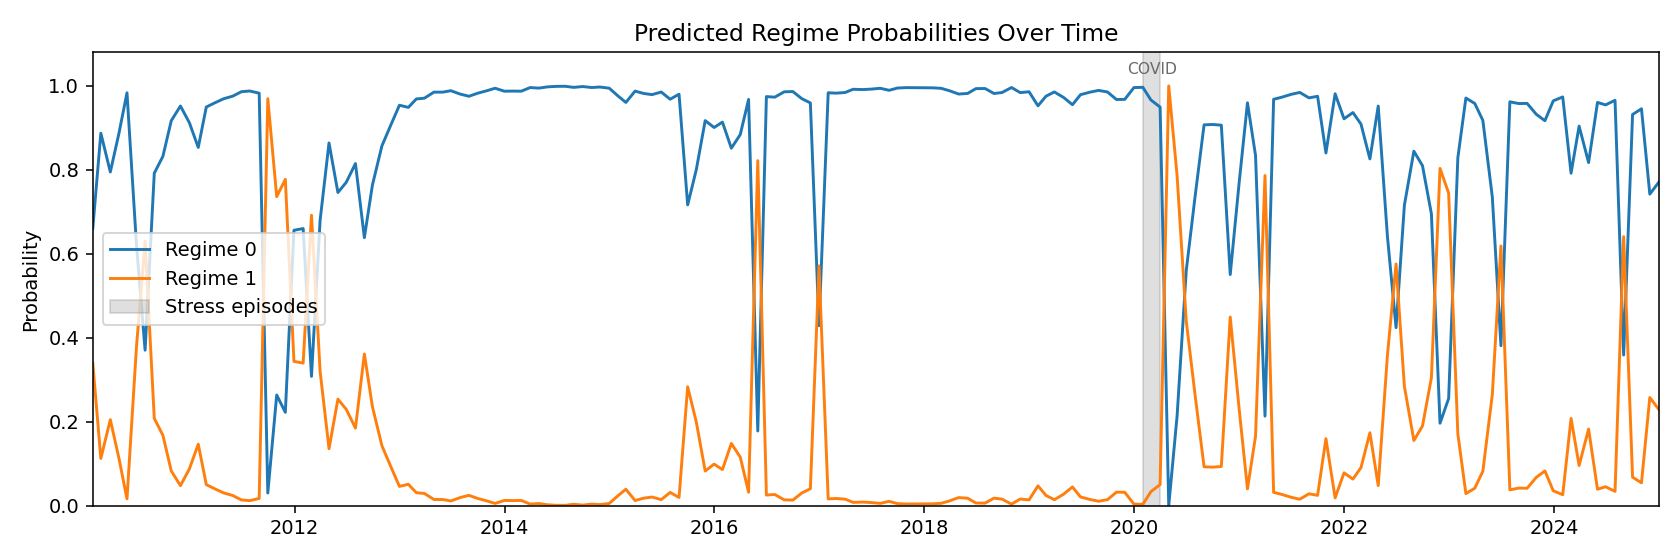
\includegraphics[width=\textwidth]{../output/figures/regime_probabilities.png}
\end{minipage}
\hfill
\begin{minipage}[t]{0.49\textwidth}
	\centering
	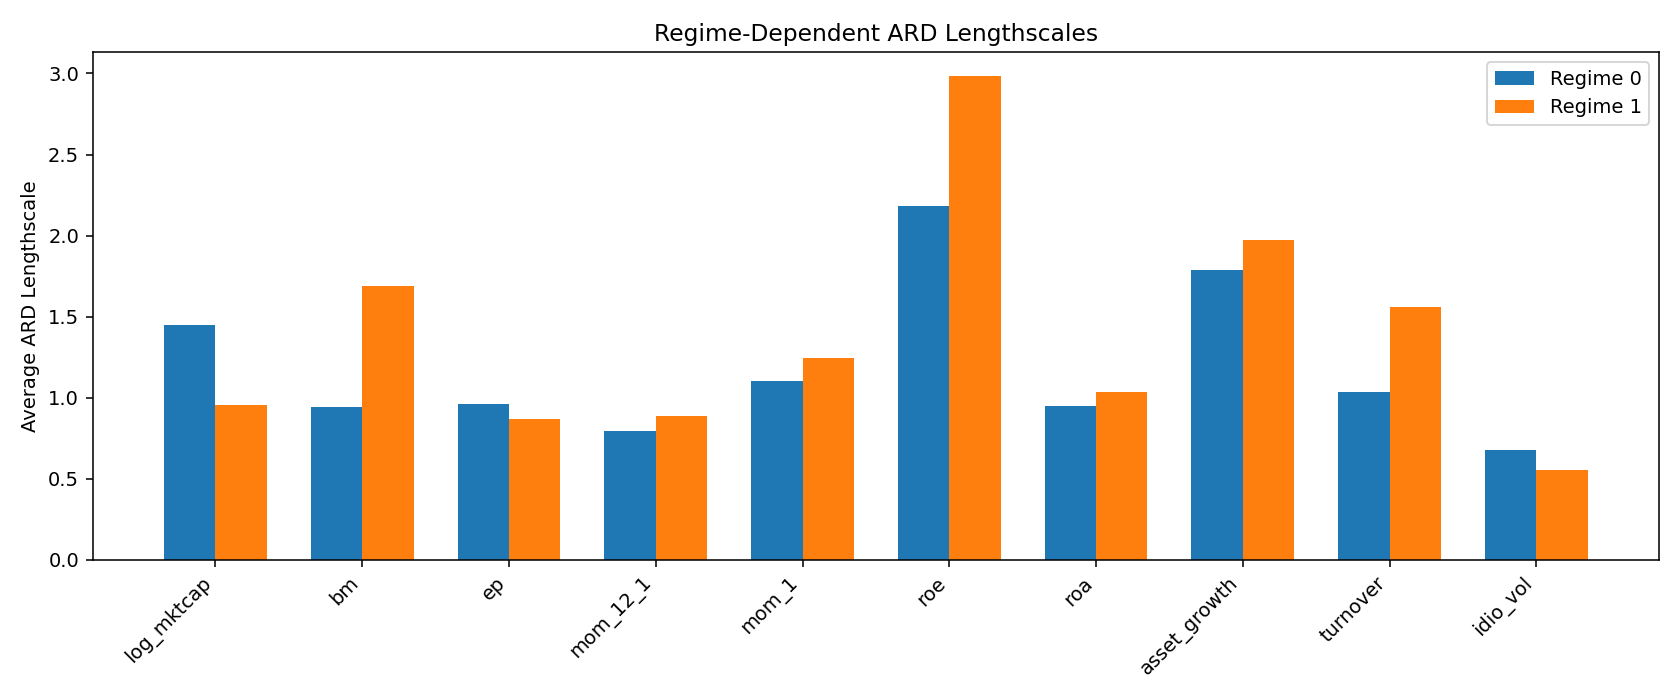
\includegraphics[width=\textwidth]{../output/figures/regime_lengthscales.png}
\end{minipage}
\caption{Estimated regime probabilities (left) and regime-specific ARD lengthscales (right).}
\label{fig:results-regime-prob-and-lengthscales}
\end{figure}
Figure 2 plots the average ARD length scale per characteristic in each regime and the inferred regime probabilities over time. Three patterns emerge that the baselines in this paper are not designed to recover jointly. The posterior probability of the high noise regime rises around the COVID shock in early 2020 and remains elevated during parts of 2022-2024. Second, several characteristics carry different importance across regimes. Third, volatility and short-run reversal carry short length scales in both regimes, indicating that they are universally informative. These rankings are the key objective that the algorithm was designed to deliver: a non-parametric result about which firm characteristics are more important and need to be part of the pricing algorithm in a certain market environment. 

To verify that macroeconomic covariates drive the transition mechanism meaningfully rather than collapsing to a constant transition matrix, we plot the fitted transition probability $P(s_t = 1|s_{t-1}, VIX_{t-1})$ as a function of lagged VIX in Appendix C. Both curves are monotonically increasing in VIX, which is the economically expected direction, as elevated implied volatility raises both the entry and persistence probabilities of the higher noise regime. This suggests that the fitted non-homogeneous transition layer is using macroeconomic information rather than collapsing to a constant transition matrix.  

\begin{table}[H]
\centering
\begin{minipage}[t]{0.43\textwidth}
\centering
\small
\textbf{Table 1: Out-of-Sample Prediction Performance}\\[4pt]
\resizebox{\linewidth}{!}{\begin{tabular}{llll}
\hline
model & oos_r2 & regime_0_r2 & regime_1_r2 \\
\hline
Fama-MacBeth & 0.0182 & 0.0155 & 0.0479 \\
RSGP & -0.0168 & -0.0107 & -0.0846 \\
Random Forest & -0.0343 & -0.0356 & -0.0193 \\
Single-Regime GP & -0.1057 & -0.1135 & -0.0197 \\
\hline
\end{tabular}}
\end{minipage}
\hfill
\begin{minipage}[t]{0.55\textwidth}
\centering
\small
\textbf{Table 2: Portfolio Performance}\\[4pt]
\resizebox{\linewidth}{!}{\begin{tabular}{lllllll}
\hline
model & ann_return & ann_vol & sharpe & capm_alpha & ff5_alpha & max_drawdown \\
\hline
RSGP & 0.2215 & 0.1332 & 1.6625 & 0.2403 & 0.2169 & -0.1775 \\
RSGP (Regime 0) & 0.2245 & 0.1342 & 1.6735 & 0.2396 & 0.2145 & -0.1543 \\
RSGP (Regime 1) & 0.1702 & 0.1217 & 1.3984 & 0.3116 & 0.2753 & -0.0301 \\
Fama-MacBeth & 0.3095 & 0.1316 & 2.3516 & 0.3275 & 0.2899 & -0.1555 \\
Random Forest & 0.2862 & 0.0972 & 2.9452 & 0.3029 & 0.2942 & -0.1001 \\
Single-Regime GP & 0.0668 & 0.0694 & 0.9635 & 0.0770 & 0.0716 & -0.1410 \\
\hline
\end{tabular}}
\end{minipage}
\label{tab:results-table-1-and-2}
\end{table}

Table 1 reports pooled out-of-sample cross-sectional $R^2$ over the 180 forecast months while table 2 shows portfolio performance (alpha ($\alpha$) comparisons presented in Appendix D). Two patterns are important:
- Fama-MacBeth attains the highest R-squared at $0.018$, while our proposed model called RSGP comes in at $-0.017$. 
- For the long-short decile portfolio, the Sharpe Ratio ordering is similar with Random Forest and Fama-Macbeth leading the way followed by our proposed RSGP model, and the single-regime GP. 
The key finding here is that RSGP does not beat every baseline model. Relative to the single regime GP, introducing regime structure roughly doubles the Sharpe ratio of a single regime GP and lifts R2 by approximately 10 percentage points while leaving the kernel family fixed. The linear and tree baselines retain an edge on the aggregate metrics, consistent with the fact that they have lower variance and the computationally constrained single-restart cold-start fitting procedure used for RSGP. The gain in portfolio performance comes from the regime switching layer that was a unique contribution of this paper and not from the GP component, which is why the single regime GP underperforms all the methods substantially. 





\section{Related Work}
\cite{filipovic_empirical_2025} is the closest paper to this project. They also apply a GP regression to the cross-section of stock returns, offering non-parametric flexibility with principled uncertainty quantification. Unlike their model, which estimates a single time-invariant pricing function, we allow the GP to switch across regimes, capturing the non-stationarity of the underlying relationship between stock returns and asset characteristics. \cite{guidolin_size_2008} show that a regime-switching linear model outperforms a single-regime linear model.

\cite{gu_empirical_2020} apply machine learning methods such as neural nets, random forests, and gradient boosting trees to show that they significantly outperform linear models for cross-sectional return prediction, establishing that non-linearity and interactions with the characteristics of the underlying asset offer better predictions. Unlike their work, we use a probabilistic regime-switching framework with GP-based uncertainty and posterior state probabilities rather than a single black box prediction function. 

\cite{jung_scalable_2022} develop scalable inference for a Bayesian hidden Markov model with GP emission models where each hidden state has its own GP with state-specific kernel hyperparameters. We inherit the core idea of regime-specific GPs governed by an HMM from them. Our work differs from theirs in two places: they target time series clustering with one-dimensional scalar inputs, while we apply it to cross-sectional asset pricing with high-dimensional characteristic vectors. They also use standard homogeneous transition probabilities, whereas to incorporate economic theory, we introduce a covariate-driven transition probability that varies.

\cite{li_hidden_2023} also apply a regime-switching GP model to time series data but they focus on electricity load forecasting. Our inference approach is inspired by theirs, where we fit HMM parameters first, then estimate per-regime GP parameters. However, unlike their work which operates on a univariate time series with seasonal structure, our setting involves a cross-section of hundreds of stocks with characteristic-driven pricing, which requires us to interpret which features are more relevant and to also model non-homogeneous transitions to capture macroeconomic regime shifts. 


\section{Limitations}
Several aspects of the model were not tested, and each one of these narrows the strength of our claims:
\begin{itemize}
	\item \textbf{Assumptions Likely Violated:} We only tested two-regime specifications, which pull together different dynamics, and finer distinctions of the pricing functions cannot be recovered. The squared exponential ARD kernel assumes a smooth pricing function, which is mis-specified for sharp threshold effects near distress. The per-period marginal likelihood reads months as conditionally independent given the regime, ignoring any serial correlation within a regime. 
	\item \textbf{When Inference Fails:} If a regime has low posterior mass, the regime-weighted GP M-step becomes ill-conditioned and loses interpretability. Similarly, transitions between regime pairs can become highly sensitive to the penalty if the multinomial logit coefficients on the macro covariates are weakly identified. 
	\item \textbf{Untested Choices:} Each month is fit with a single cold start and one restart, so we cannot rule out local optima. The M-step uses sub-sampled objectives for tractability on a local device, but it adds estimation noise of unknown magnitude. We use only 10 characteristics for each asset, rather than the broader set, which creates some inherent bias. 
	\item \textbf{Future Improvements:} Future work could explore more flexible kernels, more regimes, and alternative transition probabilities. Comparing predictive performance by running multiple EM restarts per forecast month and replacing the sub-sampled M-step with sparse GP or inducing point approximations would also be a meaningful extension. 
\end{itemize}

\section{Conclusion}
In this project, we set out to model the cross-section of expected stock returns as both non-linear and firm characteristics and non-stationary across market environments, features that the existing literature addresses one at a time but never jointly. The proposed regime-switching Gaussian process (RS-GP) model with macro-driven transitions delivers a probabilistic framework in which both of these goals are handled simultaneously. 

Three takeaways followed from the empirical analysis. First, the inference algorithm is sound; it was able to recover true regime paths and length scales on synthetic data with high accuracy. Second, the regime-switching layer is the source for the model's superior performance over a single-regime GP, roughly doubling its Sharpe ratio and lifting cross-sectional R-squared by about 10 percentage points. Third and most importantly, the regime-specific ARD lengthscales deliver an interpretable, non-parametric ranking of which firm characteristics matter for pricing in different market environments. This is novel, and no linear model, tree-based model, neural network or single-regime GP baseline can reproduce this. 

The model does not outperform every baseline on aggregate predictive measures. We are explicit that computationally constrained choices narrow the strength of our predictive claims. These limitations point to clear next steps with richer kernels, more regimes, and full sample EM with multiple restarts. The framework developed here offers a foundation that can be built upon. 



\pagebreak

\section*{Appendix A: Generalized EM Algorithm}
\begin{algorithm}[H]
\caption{Generalized EM for Regime-Switching GP Asset Pricing}
\begin{algorithmic}[1]
\Require Returns \(r_{1:T}\), characteristics \(X_{1:T}\), macro covariates \(z_{1:T}\), number of regimes \(K\)
\State Initialise the HMM with K-means on the rolling 3-month standard deviation of S\&P 500 monthly returns
\State Initialize GP hyperparameters and transition parameters
\Repeat
    \For{\(t=1,\dots,T\), \(k=0,\dots,K-1\)}
        \State Compute \(\log p(r_{t+1}\mid X_t,s_t=k)\) using the GP marginal likelihood
    \EndFor
    \State Run log-space forward-backward to obtain \(\gamma_{tk}\) and \(\xi_{t,kj}\)
    \For{\(k=0,\dots,K-1\)}
        \State Update \((\eta_k,\ell_k,\sigma_k)\) by L-BFGS on the \(\gamma\)-weighted GP marginal likelihood plus regularization
    \EndFor
    \State Update \((\alpha_{kj},\beta_{kj})\) by L-BFGS on the \(\xi\)-weighted multinomial logit objective plus ridge regularization
    \State Compute the training log-likelihood and check convergence
\Until{relative log-likelihood change is below tolerance or the iteration cap is reached}
\State Align regime labels by increasing fitted GP noise variance \(\sigma_k^2\)
\end{algorithmic}
\end{algorithm}
\pagebreak
\section*{Appendix B: Toy Data Analysis}

\begin{figure}[H]
\centering
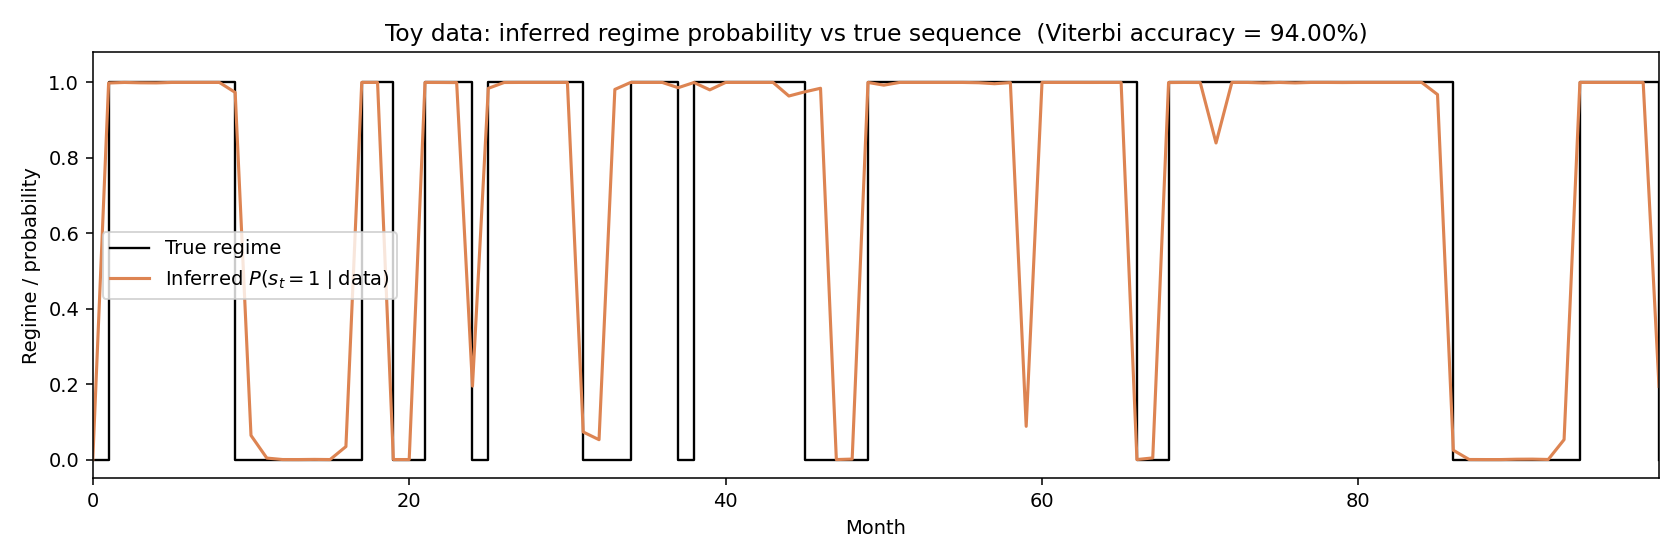
\includegraphics[width=\textwidth]{../output/figures/toy_regime_recovery.png}
\caption{Toy-data regime recovery performance.}
\label{fig:appendix-toy-regime-recovery}
\end{figure}

\begin{figure}[H]
\centering
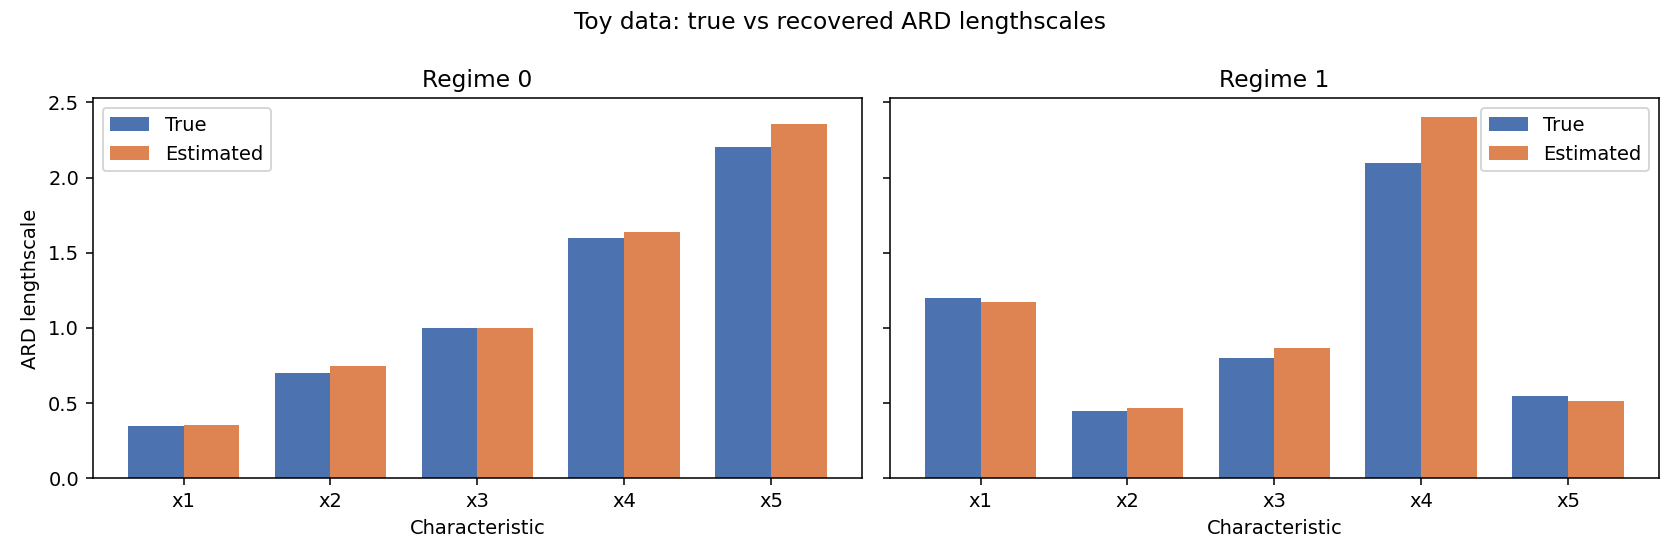
\includegraphics[width=\textwidth]{../output/figures/toy_ard_recovery.png}
\caption{Toy-data ARD lengthscale recovery.}
\label{fig:appendix-toy-ard-recovery}
\end{figure}

\pagebreak
\section*{Appendix C: Transition VIX Sensitivity}

\begin{figure}[H]
\centering
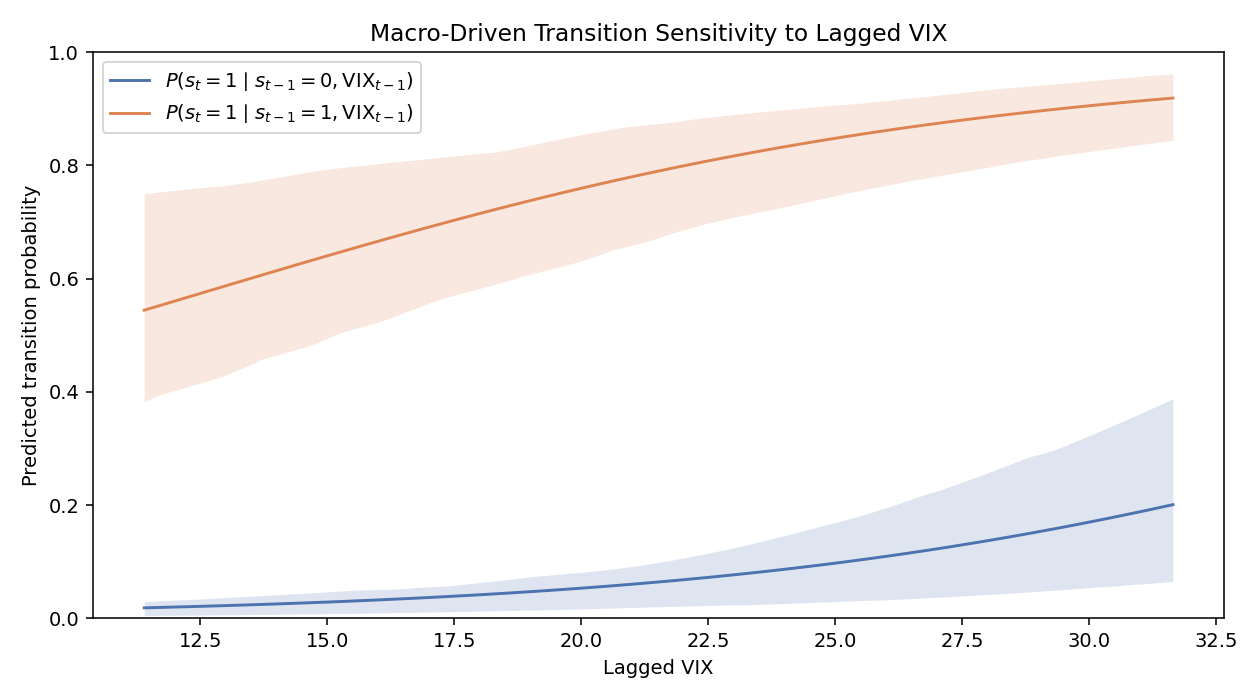
\includegraphics[width=\textwidth]{../output/figures/transition_vix_sensitivity.png}
\caption{Transition probability sensitivity to VIX.}
\label{fig:appendix-transition-vix-sensitivity}
\end{figure}

\pagebreak
\section*{Appendix D: Alpha Comparison}

\begin{figure}[H]
\centering
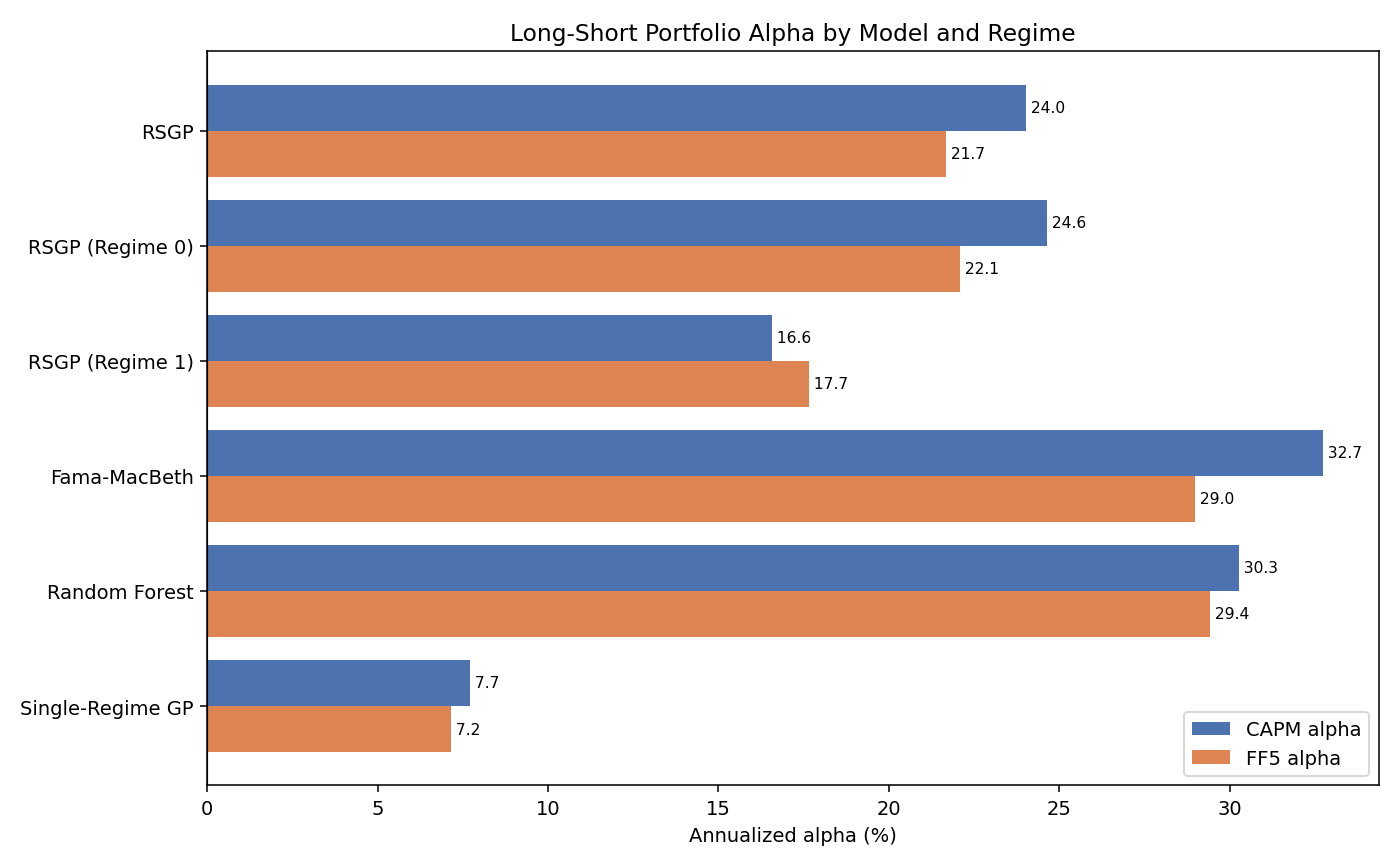
\includegraphics[width=\textwidth]{../output/figures/alpha_comparison.png}
\caption{Model alpha comparison.}
\label{fig:appendix-alpha-comparison}
\end{figure}

\pagebreak
\section*{Appendix E: Kernel Sensitivity}

\begin{figure}[H]
\centering
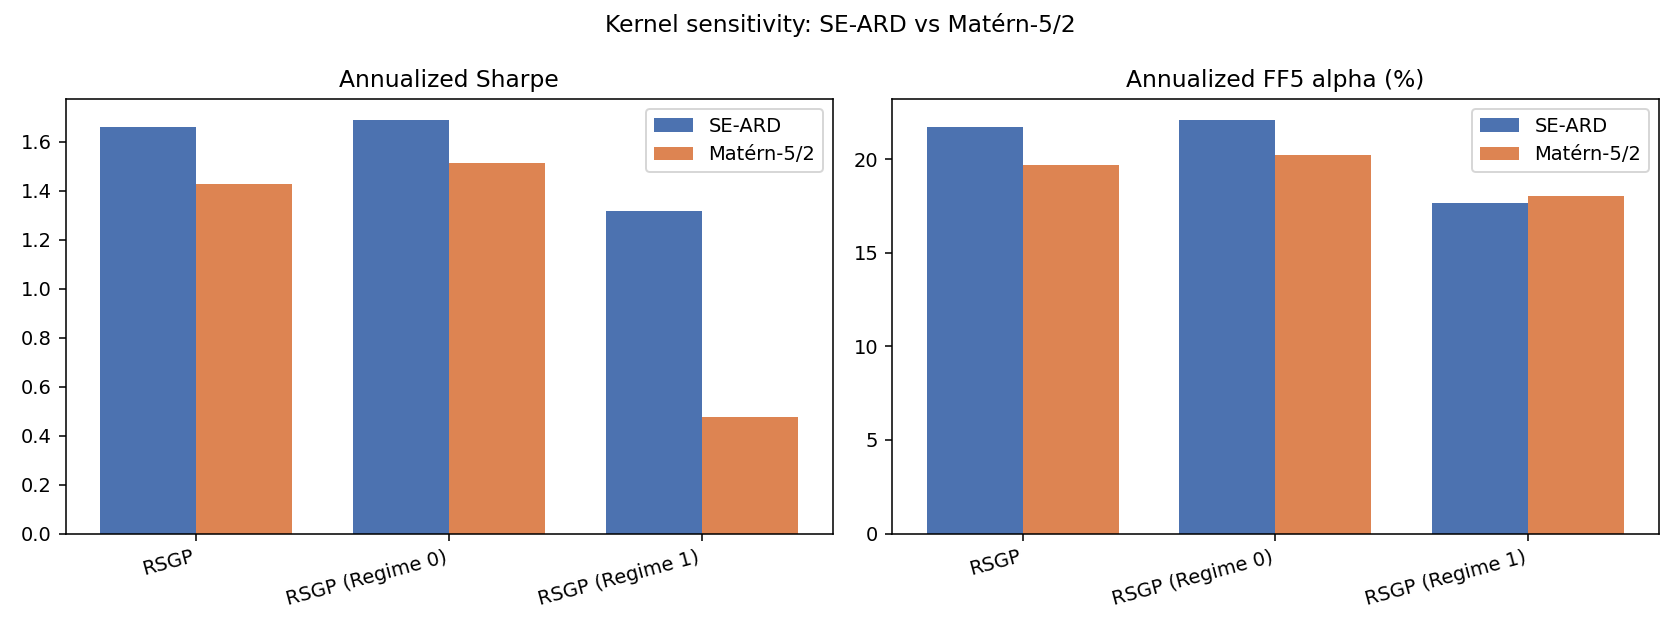
\includegraphics[width=\textwidth]{../output/figures/kernel_sensitivity.png}
\caption{Kernel sensitivity analysis.}
\label{fig:appendix-kernel-sensitivity}
\end{figure}


\pagebreak
\bibliographystyle{chicago}
\bibliography{references}

\end{document}
